¿Cuál es el perímetro del paralelogramo de la figura \ref{fig:peri_paralelogramo_02}?


% \begin{minipage}[t][][t]{0.3\textwidth}
\begin{figure}[H]
    \centering
    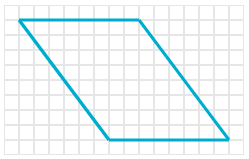
\includegraphics[width=0.2\textwidth]{../images/peri_paralelogramo_02.png}
    \caption{}
    \label{fig:peri_paralelogramo_02}
\end{figure}
% \end{minipage}\hfill
% \begin{minipage}[t][][t]{0.68\textwidth}
\begin{solutionbox}{16cm}
    \begin{minipage}{0.3\textwidth}
        \begin{figure}[H]
            \centering
            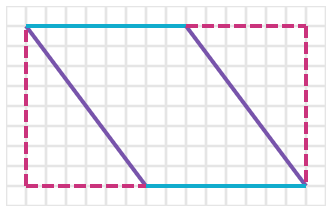
\includegraphics[width=0.6\linewidth]{../images/peri_paralelogramo_02a.png}
            \caption{}
            \label{fig:peri_paralelogramo_02a}
        \end{figure}
        \begin{figure}[H]
            \centering
            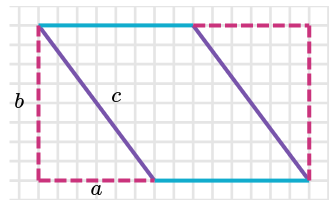
\includegraphics[width=0.6\linewidth]{../images/peri_paralelogramo_02b.png}
            \caption{}
            \label{fig:peri_paralelogramo_02b}
        \end{figure}
        \begin{figure}[H]
            \centering
            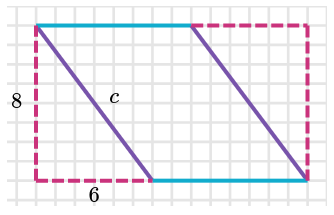
\includegraphics[width=0.6\linewidth]{../images/peri_paralelogramo_02c.png}
            \caption{}
            \label{fig:peri_paralelogramo_02c}
        \end{figure}
        \begin{figure}[H]
            \centering
            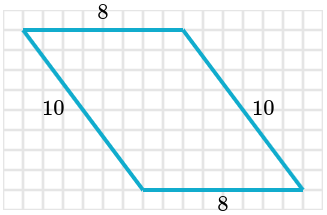
\includegraphics[width=0.6\linewidth]{../images/peri_paralelogramo_02d.png}
            \caption{}
            \label{fig:peri_paralelogramo_02d}
        \end{figure}
    \end{minipage}\hfill
    \begin{minipage}{0.65\textwidth}
        El perímetro es la distancia alrededor de una figura.
        Cada recta diagonal es la hipotenusa de un triángulo rectángulo (ver Figura \ref{fig:peri_paralelogramo_02a}).
        Podemos utilizar el teorema de Pitágoras para encontrar un lado faltante.
        La ecuación del teorema de Pitágoras es:
        \[c^2=a^2+b^2\]
        donde $a$ y $b$ son las longitudes de los catetos, y $c$ es la longitud de la hipotenusa.
        Etiquetemos la Figura del problema con $a$, $b$ y $c$ (ver Figura \ref{fig:peri_paralelogramo_02b}).
        Podemos contar los cuadrados para encontrar las longitudes de $a$ y $b$, y luego sustituir esos valores en el teorema de Pitágoras (ver Figura \ref{fig:peri_paralelogramo_02c}).
        \begin{align*}
            a^2+b^2  =c^2 & \text{\quad El teorema de Pitágoras}                          \\
            6^2+8^2  =c^2 & \text{\quad Sustituye las longitudes}                         \\
            36 +64 =c^2   & \text{\quad Evalua los cuadrados conocidos}                   \\
            100=c^2       & \text{\quad Sumando }                                         \\
            10=c          & \text{\quad Calculando la raíz en ambos lados de la ecuación} \\
        \end{align*}
        Ahora que conocemos la longitud de las diagonales, podemos encontrar la longitud de los dos lados faltantes para calcular el perímetro.
        Como los lados faltantes son rectas horizontales, podemos contar los cuadrados para obtener sus longitudes. (ver Figura \ref{fig:peri_paralelogramo_02d}).
        \[10+10+8+8=36\]
        El perímetro del paralelogramo es 36 unidades.
    \end{minipage}
\end{solutionbox}
% \end{minipage}
